\documentclass[12pt,a4paper]{article}
\usepackage{solutions-en}
\usepackage{float}

\title{Homework of 09.21\\Differential equations and dynamic systems.\\Solutions.}
\author{Глеб Минаев @ 204 (20.Б04-мкн)}
\date{}

\begin{document}
    \maketitle

    \begin{problem}{227}
        As we already know a map
        \[U(x, y) = \int \frac{dy}{f(y)} - x = \int \frac{dy}{y^{2/3}} - x = 3 y^{1/3} - x\]
        is an integral of the equation. So as far as $\lim_{y \to 0} y^{2/3}$ converges (to $0$) there will be 4 different types of solutions: for some constant $c \in \RR$ $y(c) = 0$ and to both right and left there will be 2 options $(x-c)^3$ and $0$. I.e. every solution is one of the four kinds:
        \[
            y_1(x) = (x-c)^3,
            \qquad
            y_2(x) = 0,
            \qquad
            y_3(x) =
            \begin{cases}
                (x-c)^3& \text{ if } x \geqslant c,\\
                0& \text{ if } x \leqslant c
            \end{cases}
            \qquad
            y_3(x) =
            \begin{cases}
                (x-c)^3& \text{ if } x \leqslant c,\\
                0& \text{ if } x \geqslant c.
            \end{cases}
        \]
        \begin{figure}[H]
            \centering
            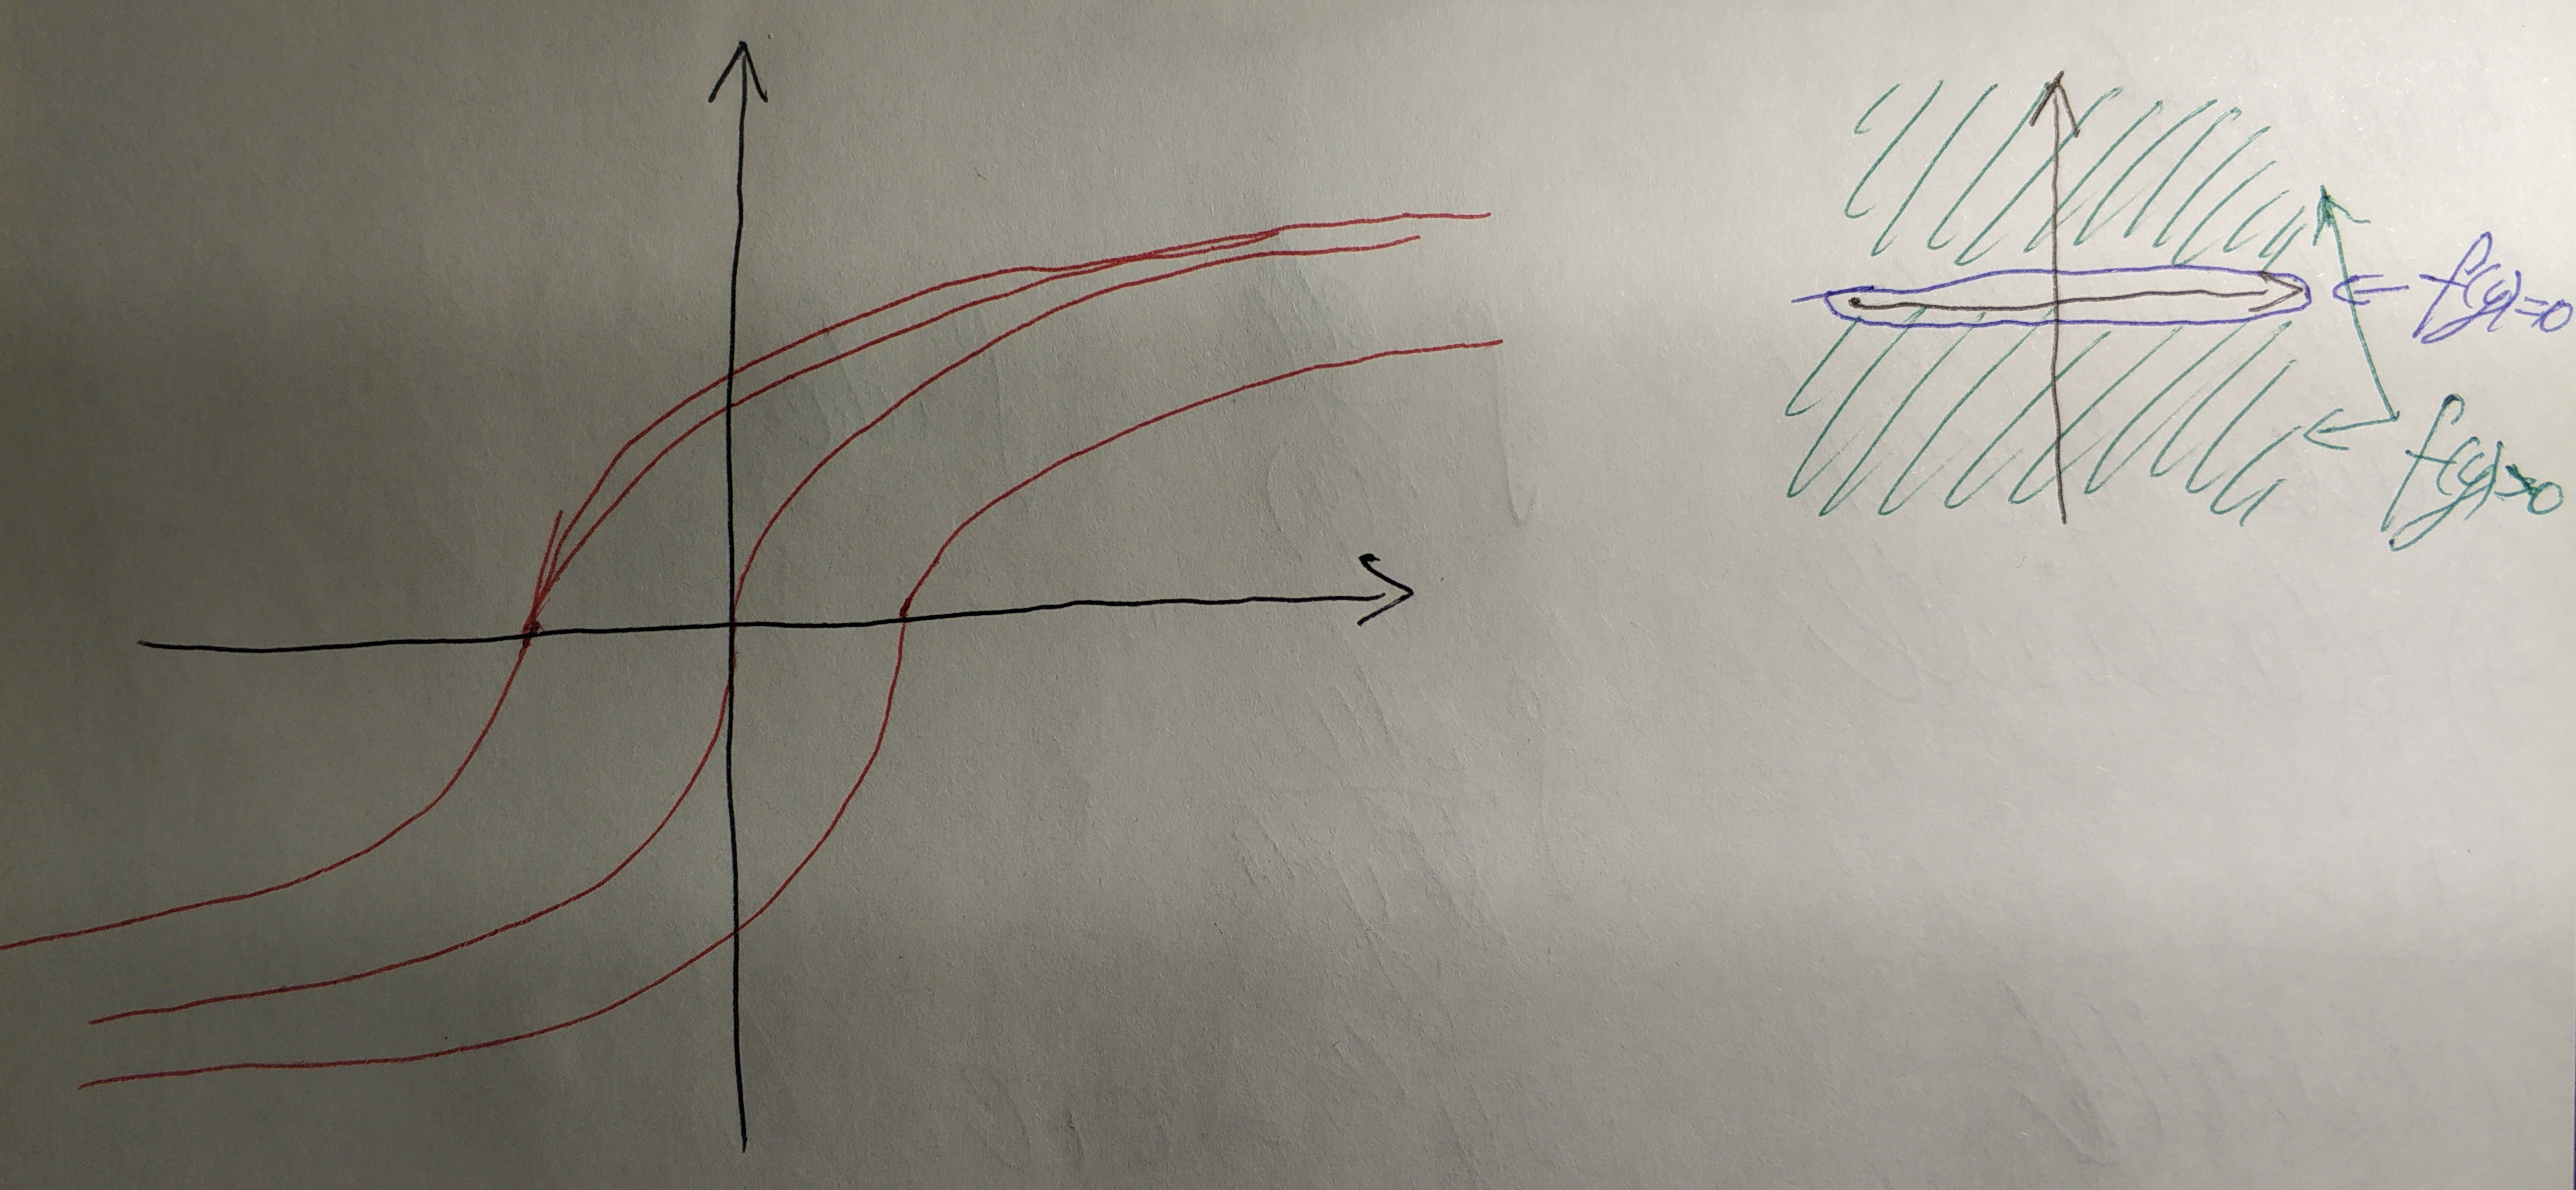
\includegraphics[height=7cm]{DEaDS-HW-003-1.jpg}
        \end{figure}
    \end{problem}

    \begin{problem}{138}
        \[y' + y \tan(x) = \frac{1}{\cos(x)}\]
        Introduce a map
        \[\varphi(x) := e^{\int_0^x \tan(t) dt} = e^{-\ln(\cos(x))} = \frac{1}{\cos(x)}.\]
        Then
        \begin{gather*}
            \varphi y' + \varphi y \tan(x) = \frac{\varphi}{\cos(x)}\\
            \varphi y' + \varphi' y = \frac{\varphi}{\cos(x)}\\
            (\varphi y)' = \frac{\varphi}{\cos(x)}\\
            \varphi y = \int \frac{\varphi(t)}{\cos(t)} dt = \int \frac{dt}{\cos(t)^2} = \tan(x) + C\\
            y = \sin(x) + C \cos(x).
        \end{gather*}
    \end{problem}

    \begin{problem}{142}
        \begin{gather*}
            2x(x^2 + y)dx = dy\\
            2x^3 + 2xy = y'\\
            y' - 2xy = 2x^3
        \end{gather*}
        Introduce a map
        \[\varphi(x) := e^{\int_0^x -2t dt} = e^{-x^2}.\]
        Then
        \begin{gather*}
            \varphi y' - \varphi 2xy = 2x^3 \varphi\\
            \varphi y' + \varphi' y = 2x^3 \varphi\\
            (\varphi y)' = 2x^3 \varphi\\
            \varphi y = \int 2t^3 \varphi(t) dt = \int 2t^3 e^{-t^2} = -(x^2 + 1)e^{-x^2} + C\\
            y = -(x^2 + 1) + C e^{x^2}.
        \end{gather*}
    \end{problem}

    \begin{problem}{149}
        \begin{gather*}
            y' = \frac{y}{3x - y^2}\\
            \frac{dy}{dx} = \frac{y}{3x - y^2}\\
            \frac{dx}{dy} = \frac{3x - y^2}{y}\\
            x' = \frac{3}{y} x - y\\
            x' - \frac{3}{y} x = -y\\
        \end{gather*}
        Introduce a map
        \[\varphi(y) := e^{\int_1^y \frac{-3}{t} dt} = e^{-3\ln(y)} = \frac{1}{y^3}.\]
        Then
        \begin{gather*}
            \varphi x' - \varphi \frac{3}{y} x = -y \varphi\\
            \varphi x' + \varphi' x = -y \varphi\\
            (\varphi x)' = -y \varphi\\
            \varphi x = \int -t \varphi(t) dt = \int \frac{-dt}{t^2} = \frac{1}{y} + C\\
            x = y^2 + C y^3.
        \end{gather*}
    \end{problem}
\end{document}